\documentclass{article}
%\documentclass[journal,transmag]{IEEEtran}
%\documentclass[10pt, conference]{IEEEtran}
\usepackage{amsmath}
\usepackage{graphicx}
%\usepackage{listings}
%\usepackage{circuitikz}
\usepackage{lscape}
\usepackage{ulem}
\usepackage{float}


\usepackage[scale=0.8]{geometry}
\begin{document}

\title{E6312: Problem Set 1}
\author{Miles Sherman}
\date{\today}
\maketitle

\section{Problem 1}
\subsubsection{Part 1}
In this simulation I aimed to plot $I_{DS}$ vs. $V_{GS}$ for my nMOS at $V_{DS} =$ 0.9V. To do this I set up a DC simulation where I swept $V_{GS}$ from 0V to 2V while plotting the current at the drain ($I_{DS}$) as my output. I chose this range because it shows the full progression of the device from weak inversion to strong inversion. My plotted output can be seen in Figure \ref{1anmos}.
\begin{figure}[\h]
\centering
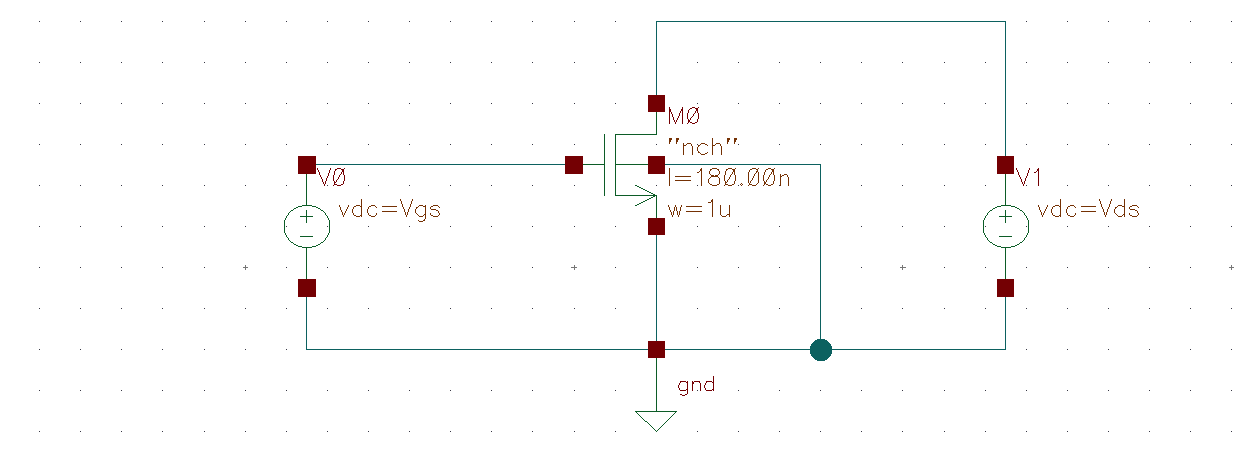
\includegraphics[width=7in]{1abc_schematic.png}
\caption{$I_{DS}$ vs. $V_{GS}$ for an nMOS at $V_{DS} =$ 0.9V}
\label{1anmos}
\end{figure}
\newpage


\end{document}
